
\begin{itemize}
\item TODO:
\begin{itemize}
    \item closure test has been repeated for pfmet in the inclusive jet bin.  
We find the uncertainty of around 15\% which seems a little bit small.  
Early this week the closure test will be repeated with the 42X MC, which should have
higher statistics and we can push the met cut a little higher and see how things evolve.
\end{itemize}
\end{itemize}

Since the production cross-section for Drell-Yan is several orders of magnitude 
higher than the $H \to ZZ$ signal, the Drell-Yan background poses a significant 
challenge. To the leading order, the Drell-Yan process does not contain \met\,  
and therefore its contribution is signficantly reduced by a tight \met selection. 
The residual Drell-Yan contribution in the signal region 
is mainly due to events with fake \met either due to energy mismeasurement of  
the hadronic recoil or momentum mismeasurement of the selected leptons. 
The contribution of events with fake \met due to the lepton momentum mismeasurement 
is expected to be small since we select events within a fairly tight (within $15$ GeV) window 
around the $Z$ boson pole mass. The background due to mismeasurement of the hadronic
recoil is the main source of Drell-Yan events contributing to the selected signal region.

The estimation of residual Drell-Yan background in the signal region depends highly on
our understanding of the \met tails which is sensitive to many factors such as 
the jet energy corrections, the number of pileup interactions, and energy from out of time
contributions. These effects are difficult to model precisely in the simulation.
Therfore we employ a data-driven method to estimate the \met distribution for the 
Drell-Yan background. For events without natural \met\, under the assumption that 
the fake \met is only resulting from mismeasurement of the hadronic recoil, we can use
$\gamma$+jets events as a control sample to predict the \met distribution in $Z$+jets
background events. If parameterized correctly in an observable that is highly correlated 
with the source of fake \met, one expects $\gamma$+jets events to provide an accurate
model of the \met distribution for $Z$+jets events, provided that the photon
is well measured and does not contribute to the \met.

\subsubsection{Photon Selection and Reweighting Procedure}
The photon data sample is selected by requiring one and only one photon passing reaonsably tight
identification and isolation requirements, summarized in Table \ref{tab:PhotonSelection} below 
\cite{MITHggNote}. 
An electron veto is imposed on the photon, requiring that the photon is not matched to a pixel seed.
To reduce contamination from $W$+$\gamma$ events, we veto any events with one or 
more well identified leptons.


\begin{table}[!ht]
\begin{center}
\begin{tabular}{|c|c|} 
\hline
Cut           & Requirement                                                                           \\
\hline
\multicolumn{2}{|c|}{Photon is not pixel seeded}                                                      \\
\hline
$\eta$        & $|\eta| < 1.4442$                                                                     \\ 
\hline
H/E           & H/E $< 0.05$                                                                          \\
$\sigma_{i\phi i\phi}$ & $\sigma_{i\phi i\phi} > 0.001$                                           \\
$\sigma_{i\eta i\eta}$ & $0.001 < \sigma_{i\eta i\eta} < 0.013$                                   \\
\hline
EcalIso       & EcalIso $<  4.2 + 0.0060\times p_{T}$   \\
HcalIso       & HcalIso $<  2.2 + 0.0025\times p_{T}$  \\
TrkIso        & TrkIso  $<  2.0 + 0.0010\times p_{T}$     \\
\hline
%Electron Veto & Photon is rejected if it shares the supercluster with an electron that does not       \\
%              & match to one leg of a conversion with $\mathrm{L}_{\mathrm{xy}} < 2.0$, fit           \\
%              & probability  $> 10^{-6}$, and no hits behind the fitted vertex                        \\
%\hline
%\hline
%\multicolumn{2}{|c|}{Conversion ID (if matched to a conversion with $\mathrm{L}_{\mathrm{xy}} < 2.0$,}\\
%\multicolumn{2}{|c|}{fit probability $> 10^{-6}$, and at most one hit before the fitted vertex on }   \\
%\multicolumn{2}{|c|}{either of the tracks forming the conversion) }                                   \\
%\hline
%E/P            & E/P $< 2.0 $                                                                         \\
%$\Delta\eta$  & $|\Delta\eta| < 0.01 for Endcap only$ \\
%$\Delta\phi$  & $|\Delta\phi| < 0.01 for Endcap only$ \\
%\hline
%\hline
%\multicolumn{2}{|c|}{Isolation}                                                                       \\
%\hline
%EcalIso       & EcalIso $ - \rho\times \mathrm{A}_{\mathrm{eff Ecal}}$ $<  2.0 + 0.006\times p_{T}$   \\
%HcalIso       & HcalIso $ - \rho\times \mathrm{A}_{\mathrm{eff Hcal}}$ $<  2.0 + 0.0025\times p_{T}$  \\
%TrkIso        & TrkIso $ - \rho\times \mathrm{A}_{\mathrm{eff Trk}}$ $<  1.5 + 0.001\times p_{T}$     \\
%\hline

%\hline
%SpikeKilling & \\
%\hline
%$E_{\mathrm{Max}} / E_{9}$ & $E_{\mathrm{Max}} / E_{9} > 0.95$       \\
%$\sigma_{i\eta i\eta}$     & $\sigma_{i\eta i\eta} > 0.001$          \\
%$\sigma_{i\phi i\phi}$     & $\sigma_{i\phi i\phi} > 0.001$          \\
%\hline
\end{tabular}
\caption{The selection criteira on the photons.
\label{tab:PhotonSelection}}
\end{center}
\end{table}

To ensure the photon is well-measured in both the online HLT reconstruction as well as the offline reconstruction, we require that photons in
various $p_T$ ranges be accepted by specific triggers as listed in Table~\ref{tab:PhotonTriggerPtBins}. The $p_T$ bins are motivated by the
desire to avoid the turn-on regions of the various triggers.
\begin{table}[!ht]
\begin{center}
\begin{tabular}{|c|c|} 
\hline
$p_T$ range     & Trigger requirement \\
\hline
$25 < p_T < 35$ & HLT\_Photon20\_* \\
$35 < p_T < 55$ & HLT\_Photon30\_* \\
$55 < p_T < 80$ & HLT\_Photon50\_* \\
$80 < p_T < 95$ & HLT\_Photon75\_* \\
$p_T > 95$      & HLT\_Photon90\_* \\
\hline
\end{tabular}
\caption{The selection criteira on the photons.
\label{tab:PhotonTriggerPtBins}}
\end{center}
\end{table}

Since the fake \met is due to mismeasurement of the hadronic recoil, we parameterize the 
modelling of the \met distribution in the $p_{T}$ of the photon / dilepton system and 
the number of counted jets. Both variables are highly correlated with the behavior 
of the hadronic recoil. Additionally, since the photon triggers are prescaled
the photon events are sampling the pile-up conditions differently than the events which
pass selection. To address this, we parametrize also in the vertex multiplicity.
Reweighting factors are computed in bins of the number of counted jets
and the dilepton $p_{T}$, and in the number of primary vertices,
by dividing the corresponding two dimensional distributions
in the $\gamma$+jets data sample and the dilepton data sample:

\begin{eqnarray}
  w(p_{T},\mathrm{njet}) = \frac{\mathrm{N}_{\gamma+\mathrm{jets}}(p_{T},\mathrm{njet})}{\mathrm{N}_{\mathrm{Z+jets}}(p_{T},\mathrm{njet})}
  \times\frac{\mathrm{N}_{\gamma+\mathrm{jets}}(\mathrm{npv})}{\mathrm{N}_{\mathrm{Z+jets}}(\mathrm{npv})}.
\end{eqnarray}

In order for these reweighting factors to be insensitive to the presence of signal or backgrounds with 
real \met, we build these weight factors on a $\gamma$+jets and $Z$+jets sample by
requiring the \met to be below $50$ GeV. For the $Z$+jets sample, 
the full $H \to ZZ$ preselection is imposed, including the top veto and the third lepton veto.

Finally, to model the \met distribution for the final selection we select $\gamma$+jets events
as above, imposing the preselection requirement that the photon $p_{T}$ is greater than $25$ GeV,
and associate the corresponding weight factor $w(p_{T},\mathrm{njet},\mathrm{npv})$ to each such event. 
To model the transverse mass distribution, we draw a random number from a pre-determined dilepton
mass distribution and build the $m_{T}$ observable as in Eqn \ref{eq:MTHZZ}. The dilepton mass distribution
is constructed from data imposing all preselection cuts except the $\met\ $ requirement.

\subsubsection{Monte Carlo Closure Test}

In order to verify that the procedure models the $Z$+jet background well, we test it
in $\gamma$+jets and $Z$+jets Monte Carlo simulation. The reweighting factors are 
built from the simulation sample according to the procedure described above and then 
applied on the $\gamma$+jets Monte Carlo sample. 

In Fig \ref{fig:PhotonJetsClosureTest} we show the particle flow \met distribution 
from the $\gamma$+jet sample after reweighting compared to the \met distribution from the 
$Z$+jet sample, separately in the 0-jet, 1-jet, and 2-jet bins. We observe agreement between 
the $\gamma$+jet generated prediction and the $Z$+jet simulation particle flow \met distribution. 

\begin{figure}[!htbp]
\begin{center}
\subfigure[0-Jet]{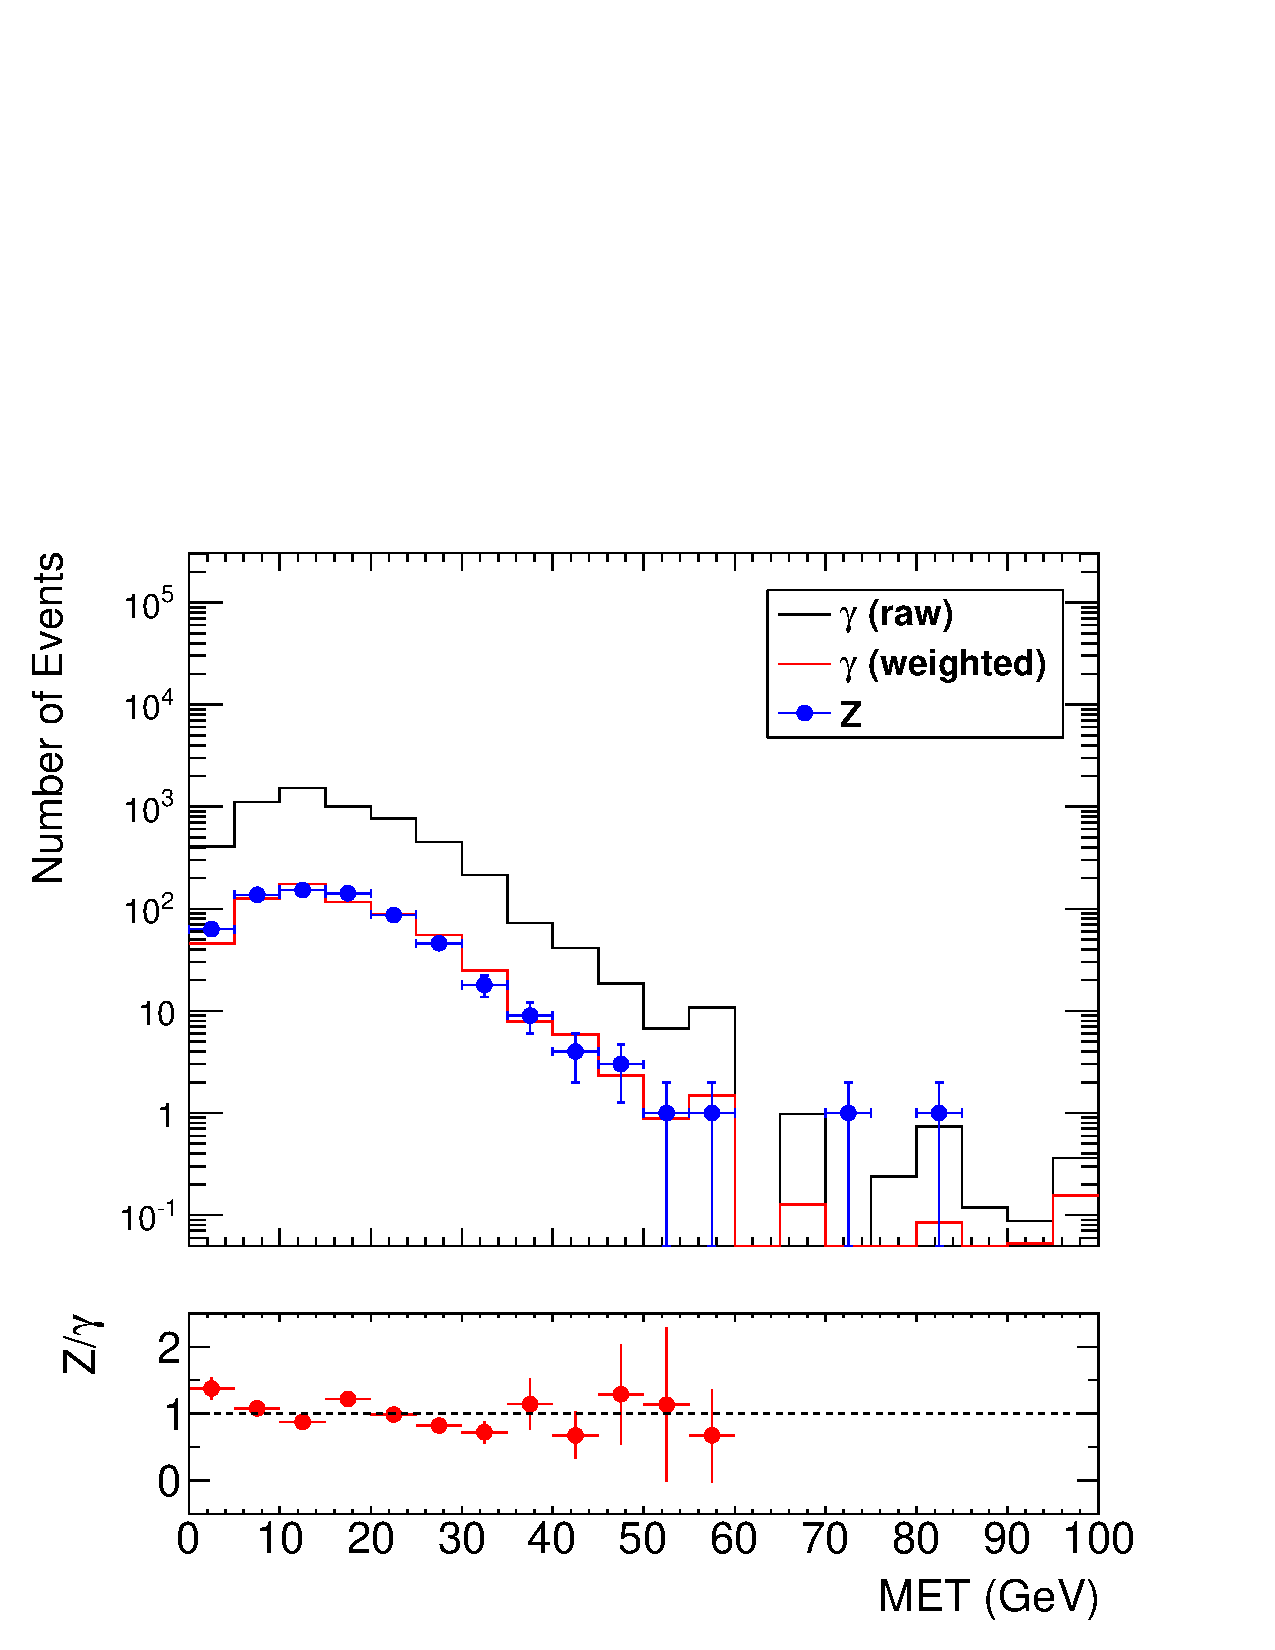
\includegraphics[width=0.49\textwidth]{figures/results_met_41X_MC_all_0j_met.pdf}}
\subfigure[1-Jet]{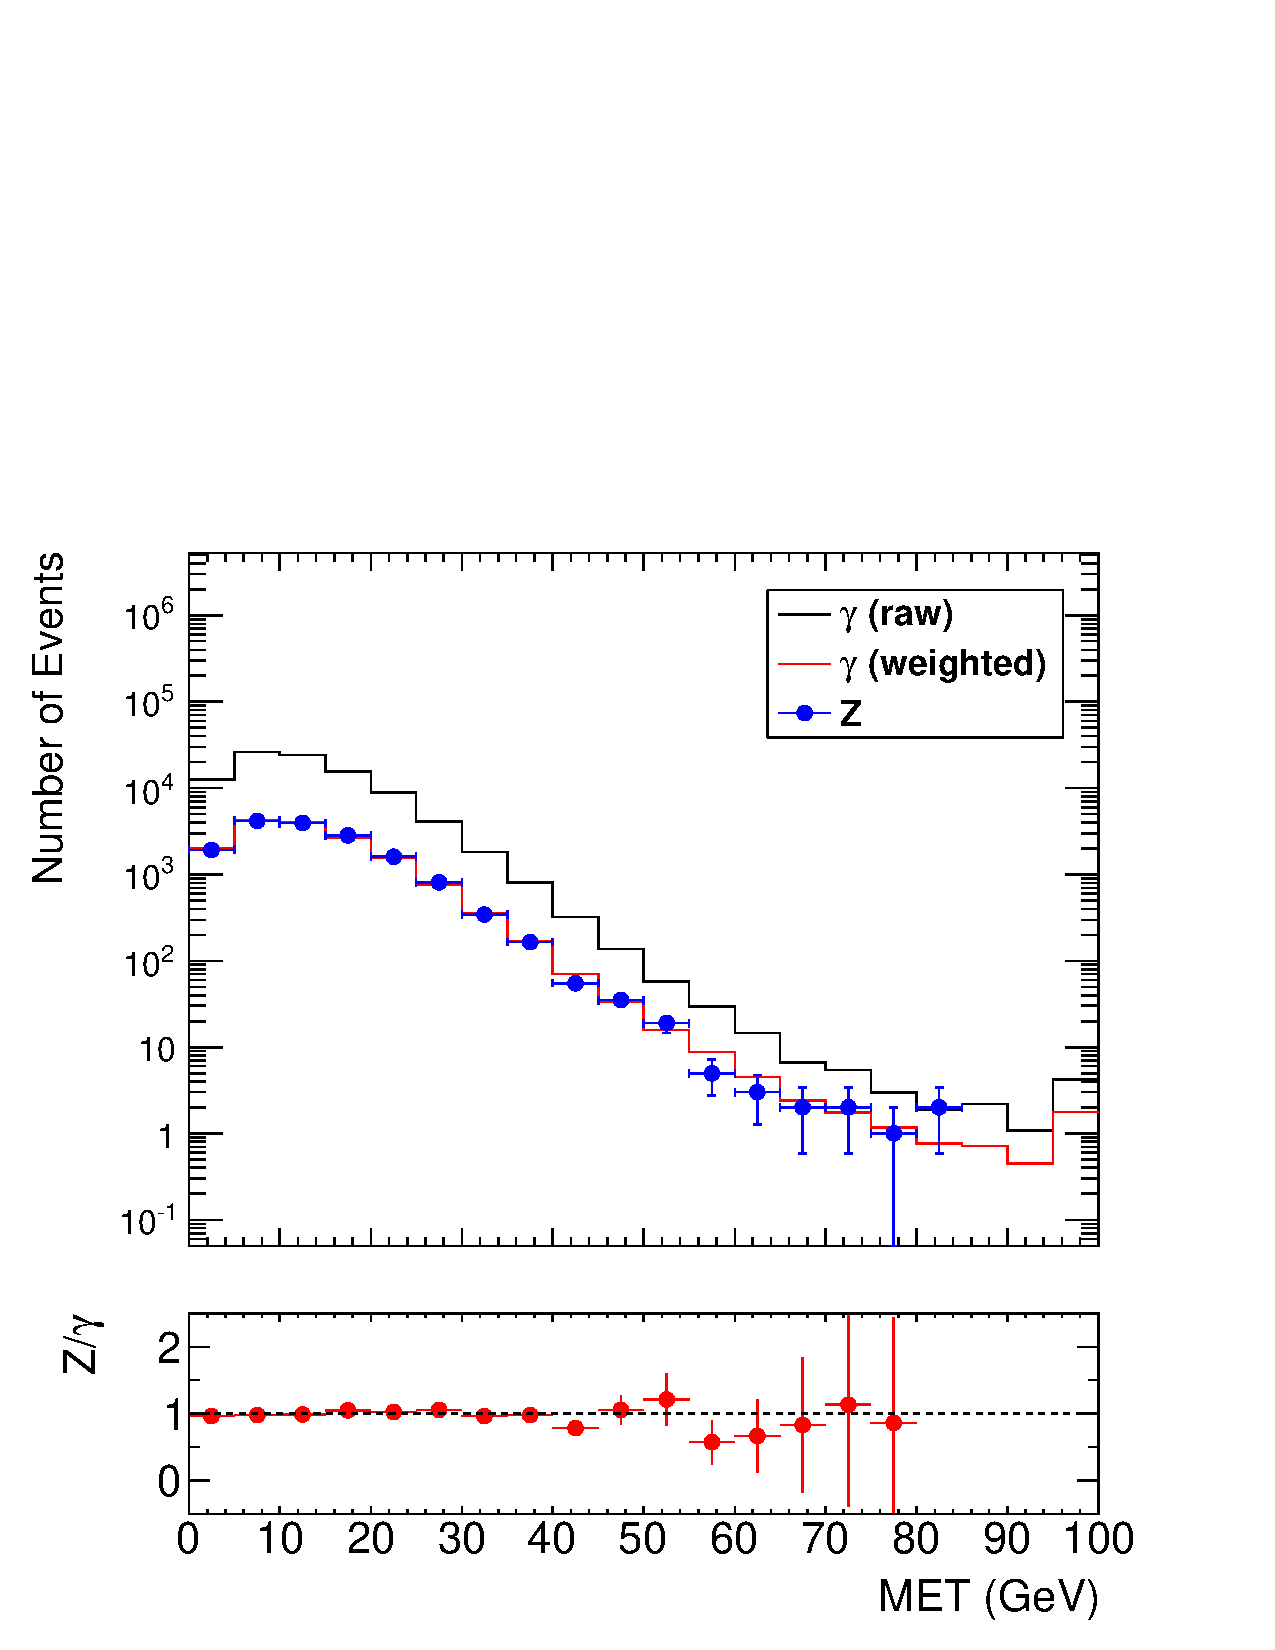
\includegraphics[width=0.49\textwidth]{figures/results_met_41X_MC_all_1j_met.pdf}}
\subfigure[2-Jet]{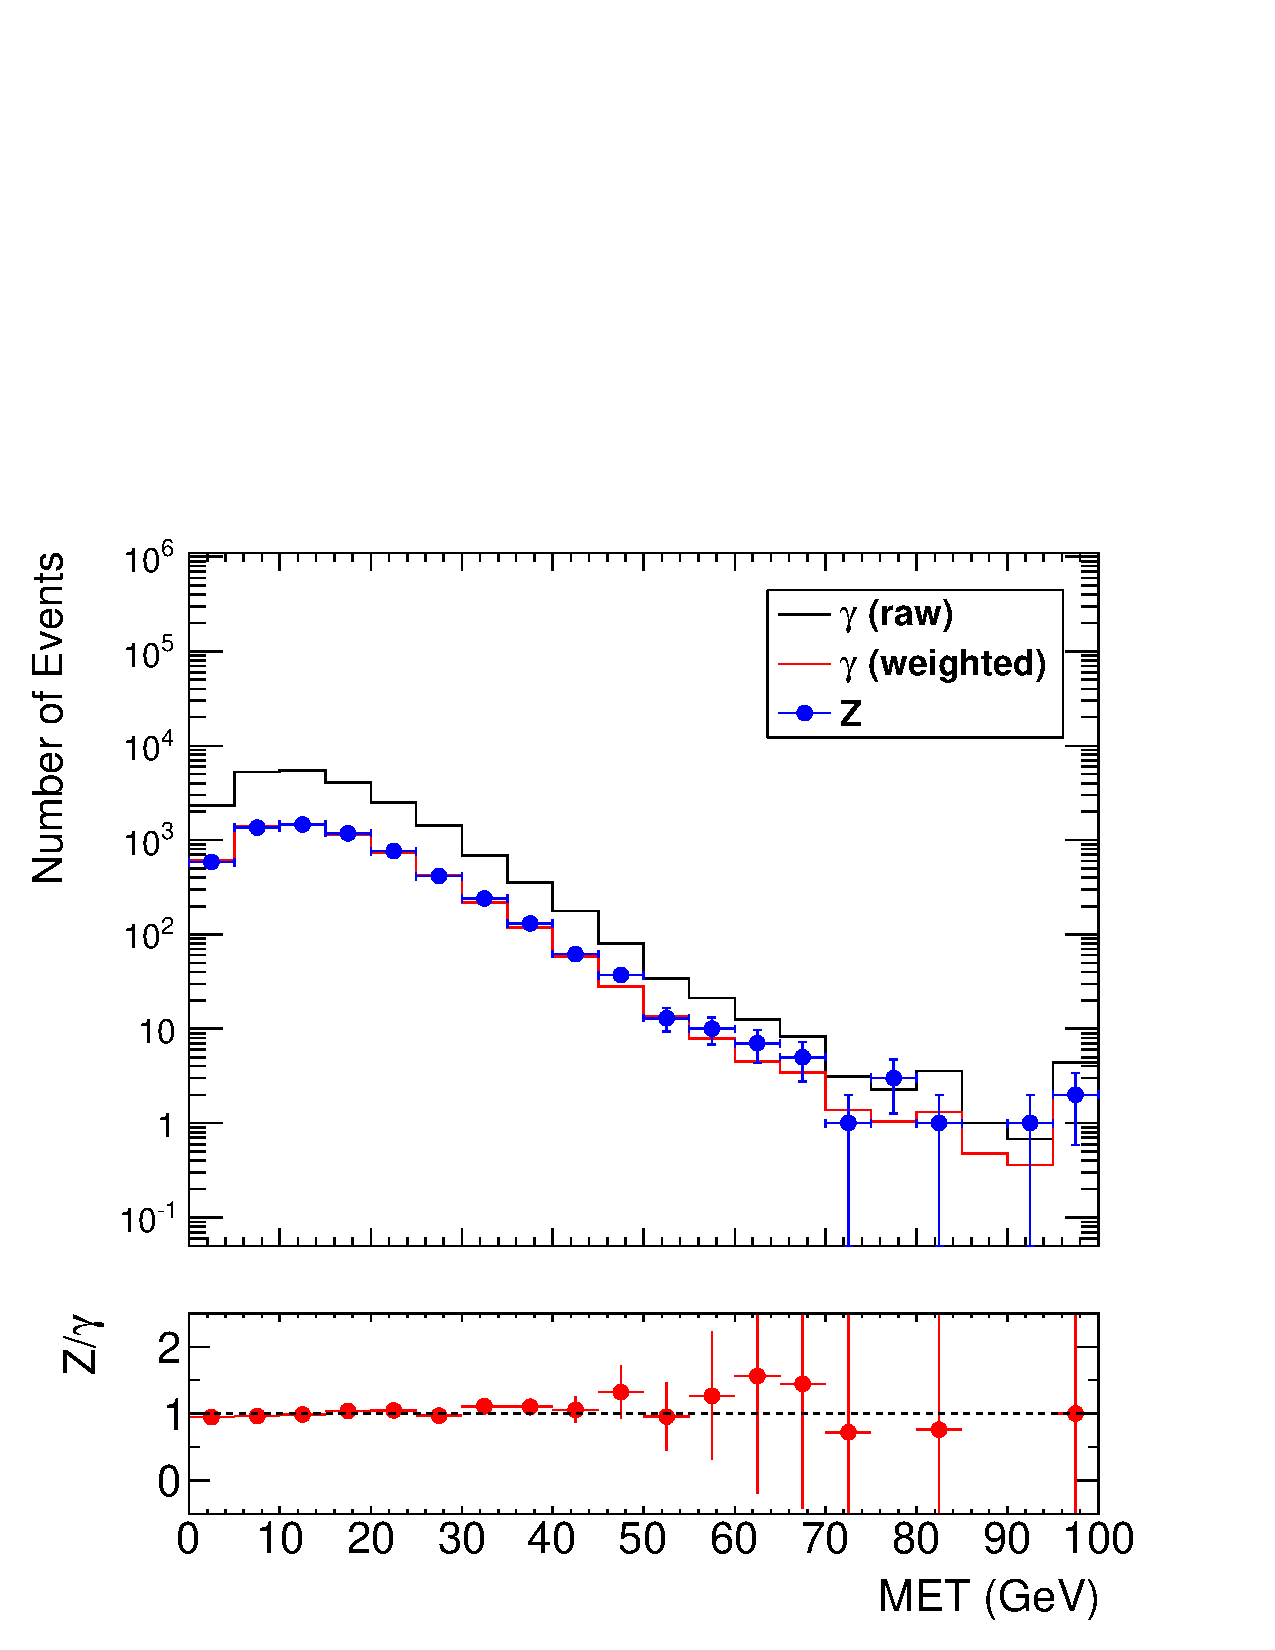
\includegraphics[width=0.49\textwidth]{figures/results_met_41X_MC_all_2j_met.pdf}}
\subfigure[Inclusive]{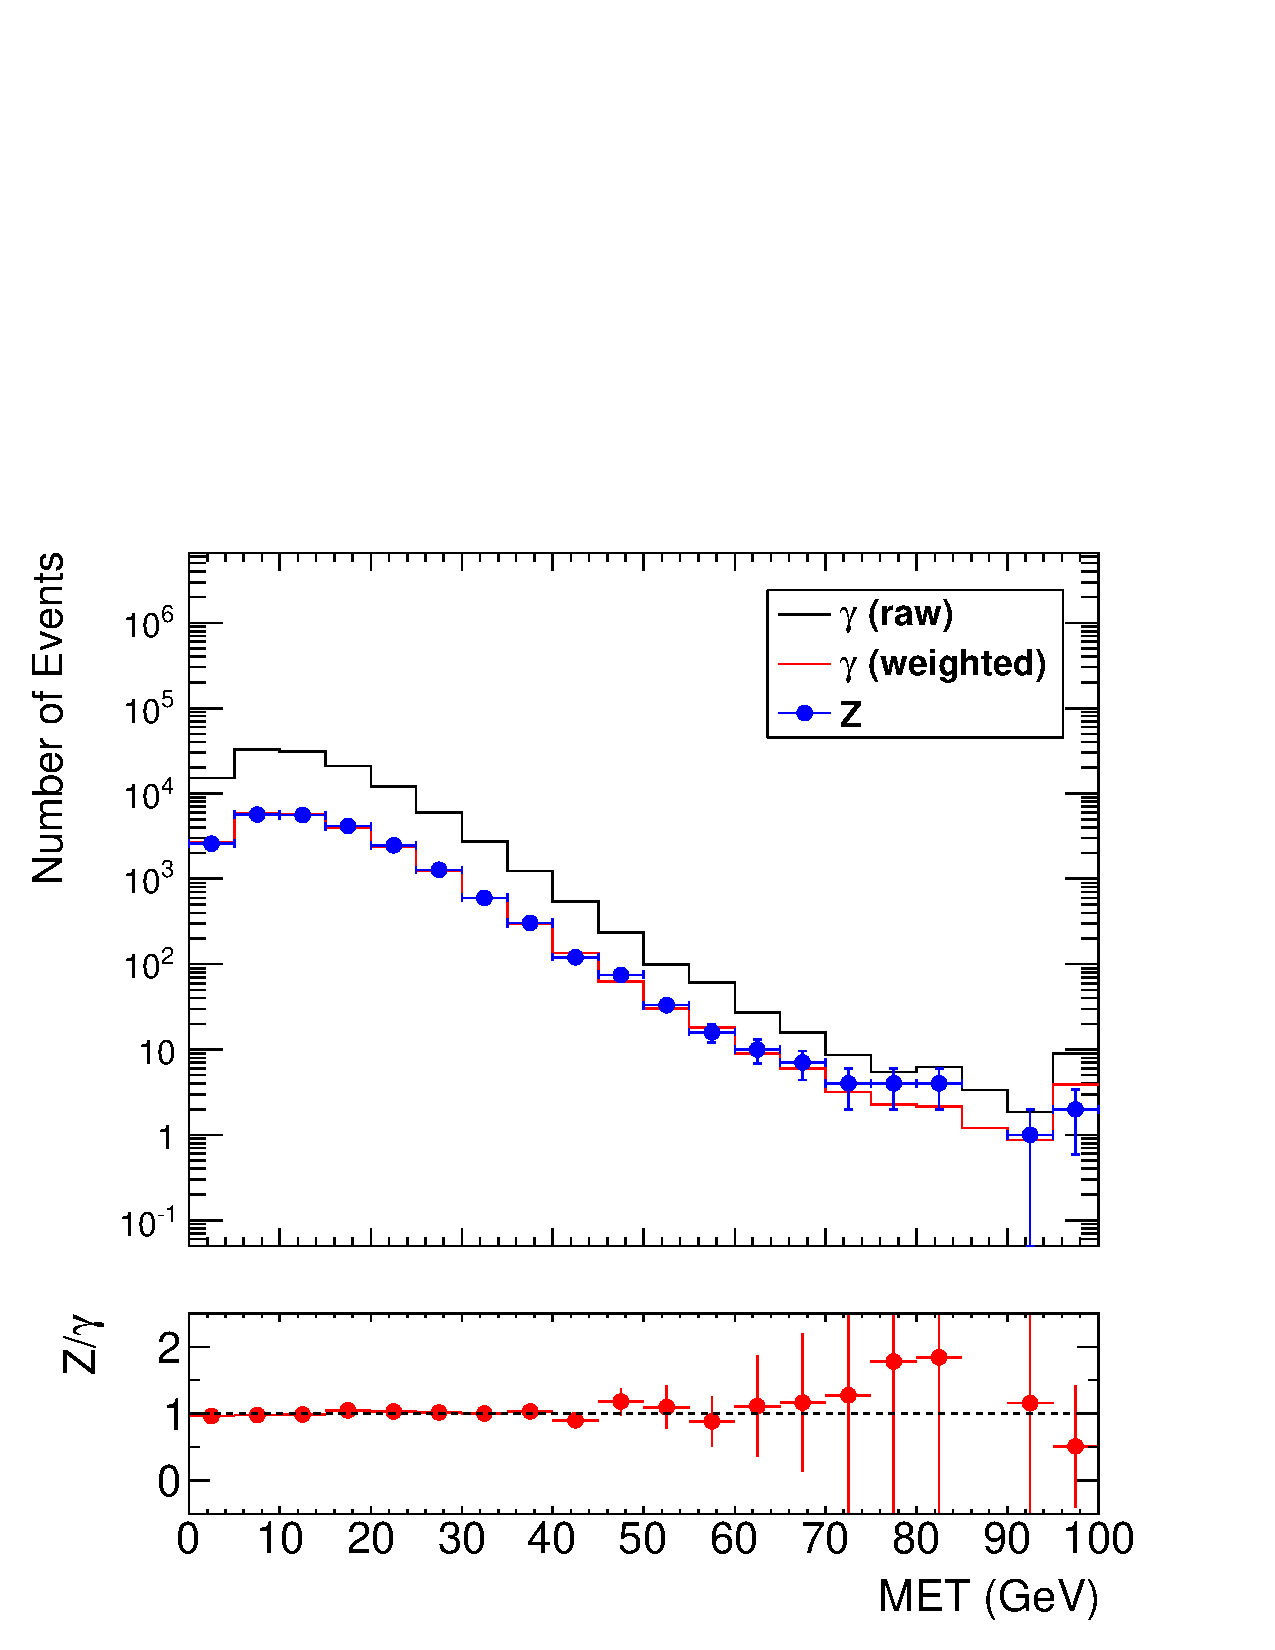
\includegraphics[width=0.49\textwidth]{figures/results_met_41X_MC_all_incl_met.pdf}}
\caption{Comparison of the particle flow \met prediction from the reweighted $\gamma$+jets sample
and the simulation prediction from the $Z$+jets sample.}
\label{fig:PhotonJetsClosureTest}
\end{center}
\end{figure}

\begin{figure}[!htbp]
\begin{center}
%\subfigure[0-Jet]{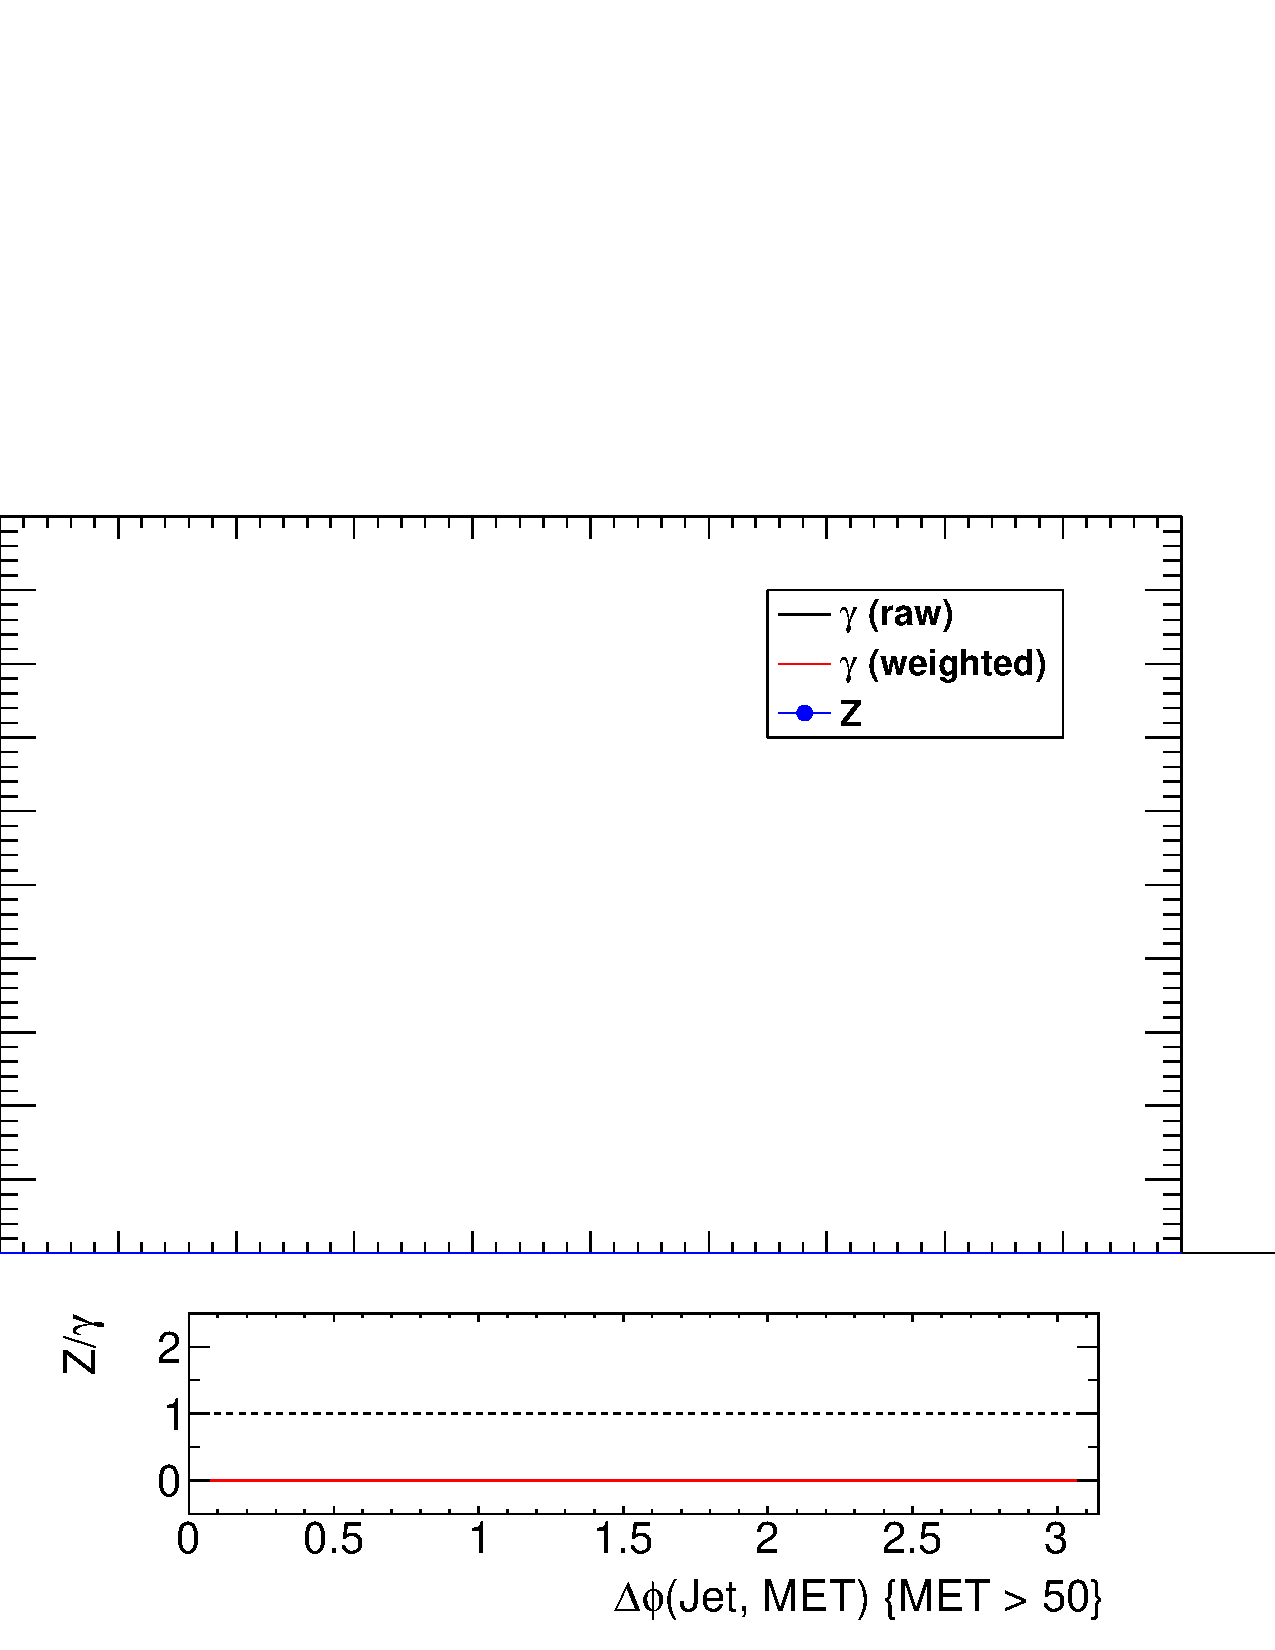
\includegraphics[width=0.4\textwidth]{figures/results_met_41X_MC_all_0j_dphi.pdf}}
\subfigure[1-Jet]{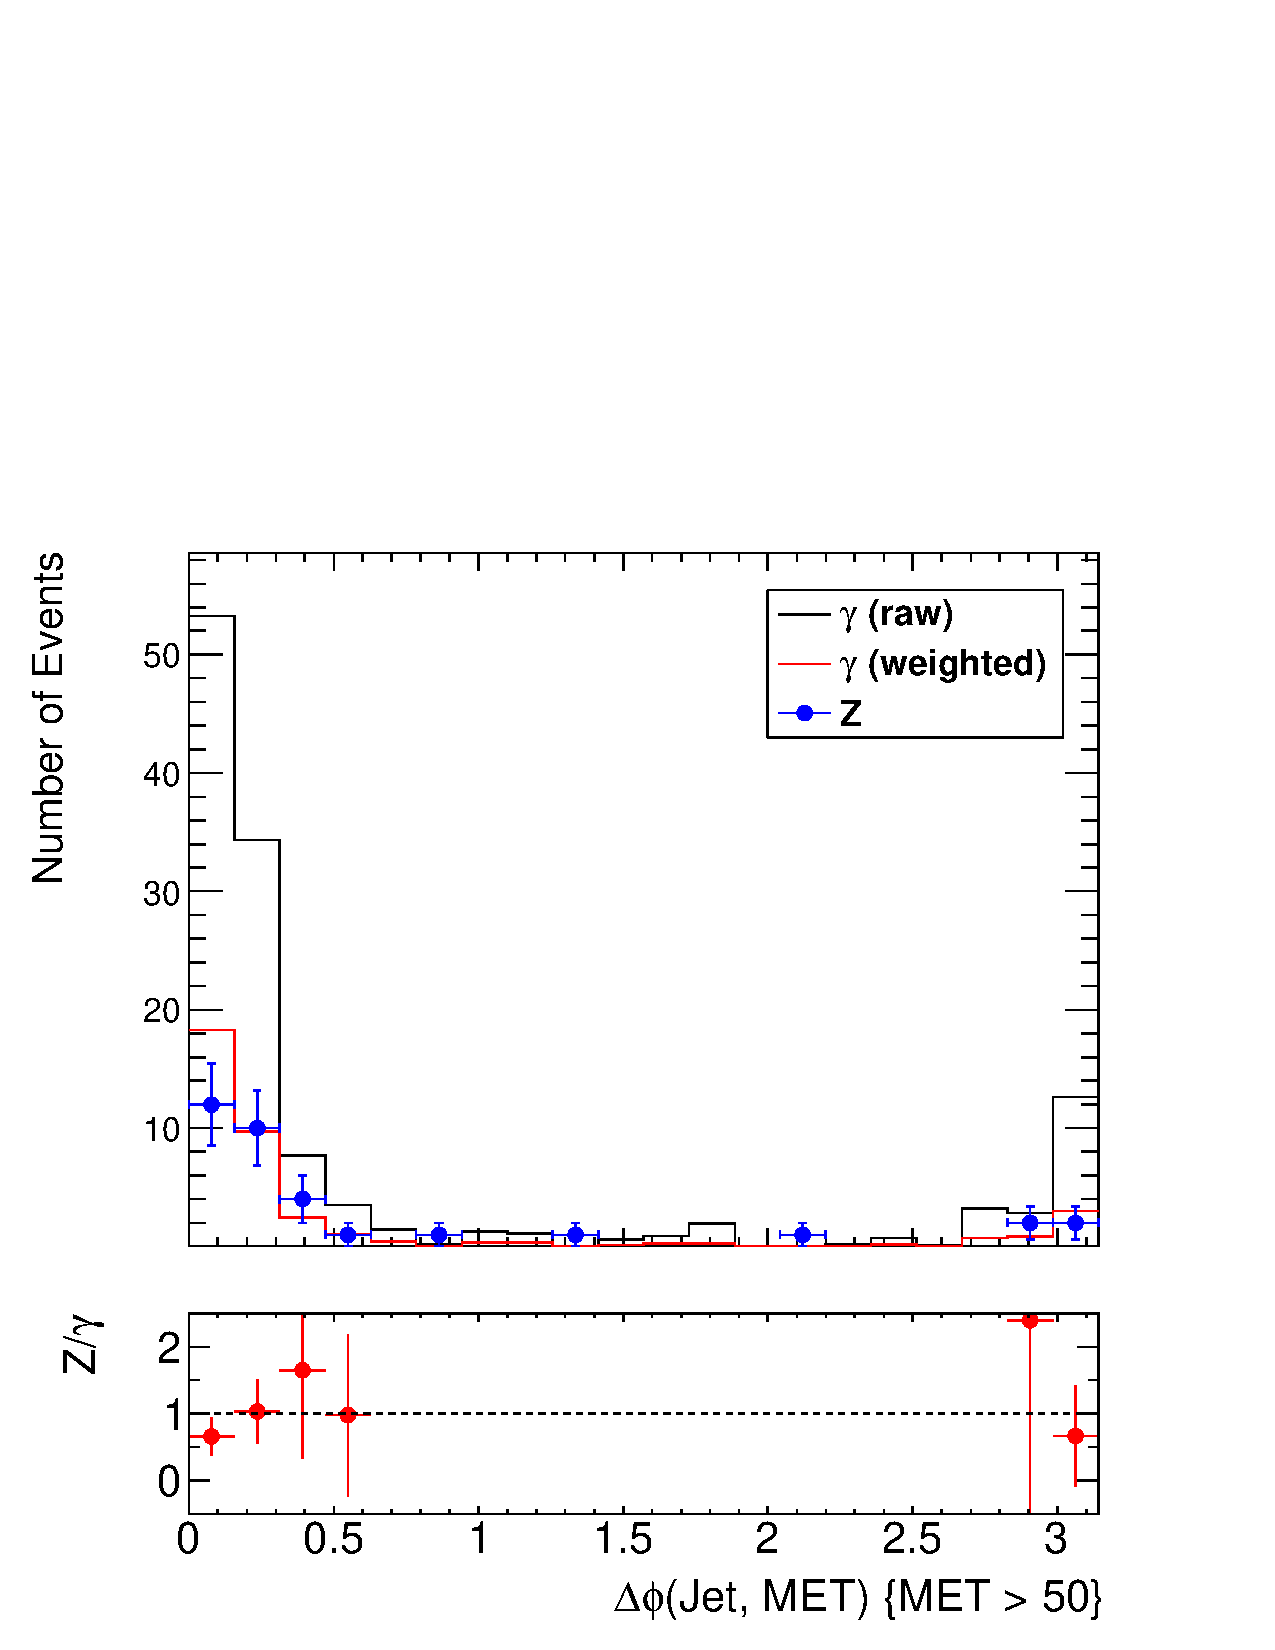
\includegraphics[width=0.49\textwidth]{figures/results_met_41X_MC_all_1j_dphi.pdf}}
\subfigure[2-Jet]{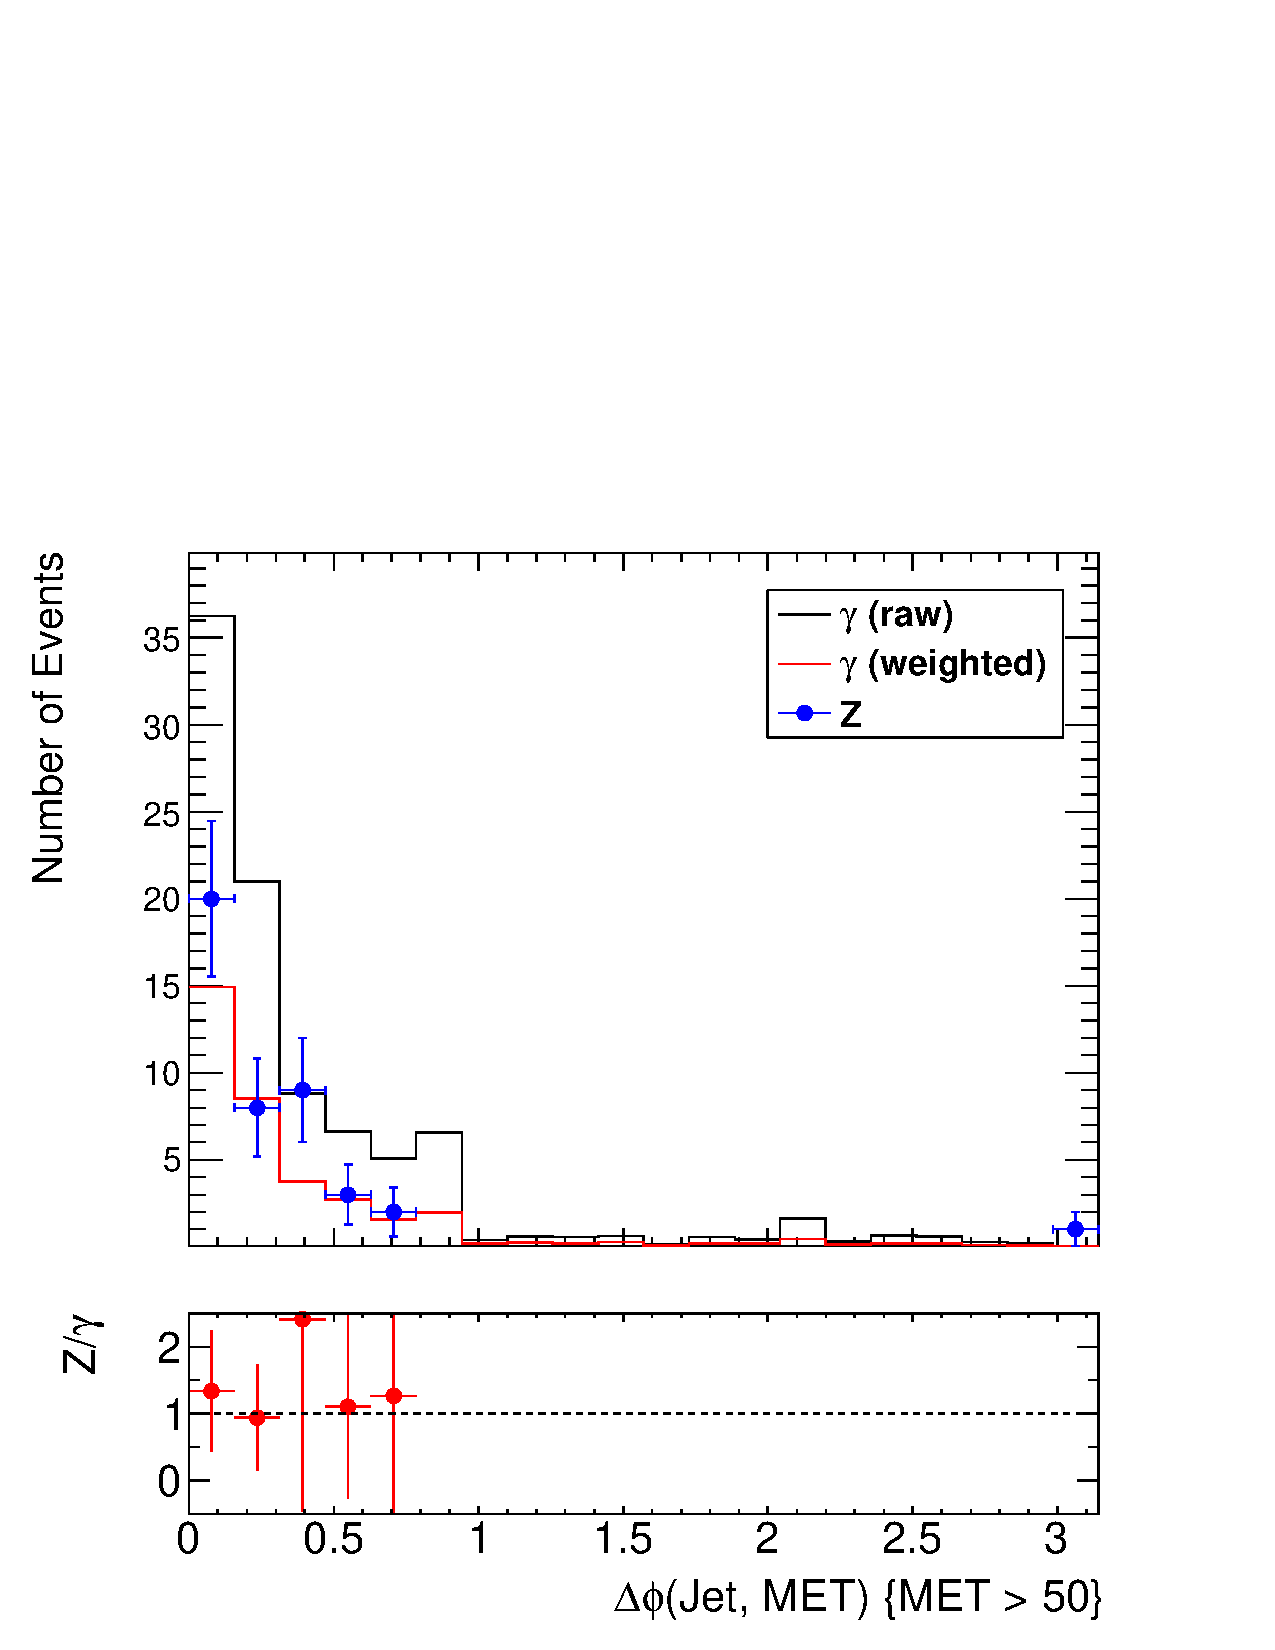
\includegraphics[width=0.49\textwidth]{figures/results_met_41X_MC_all_2j_dphi.pdf}}
\subfigure[Inclusive]{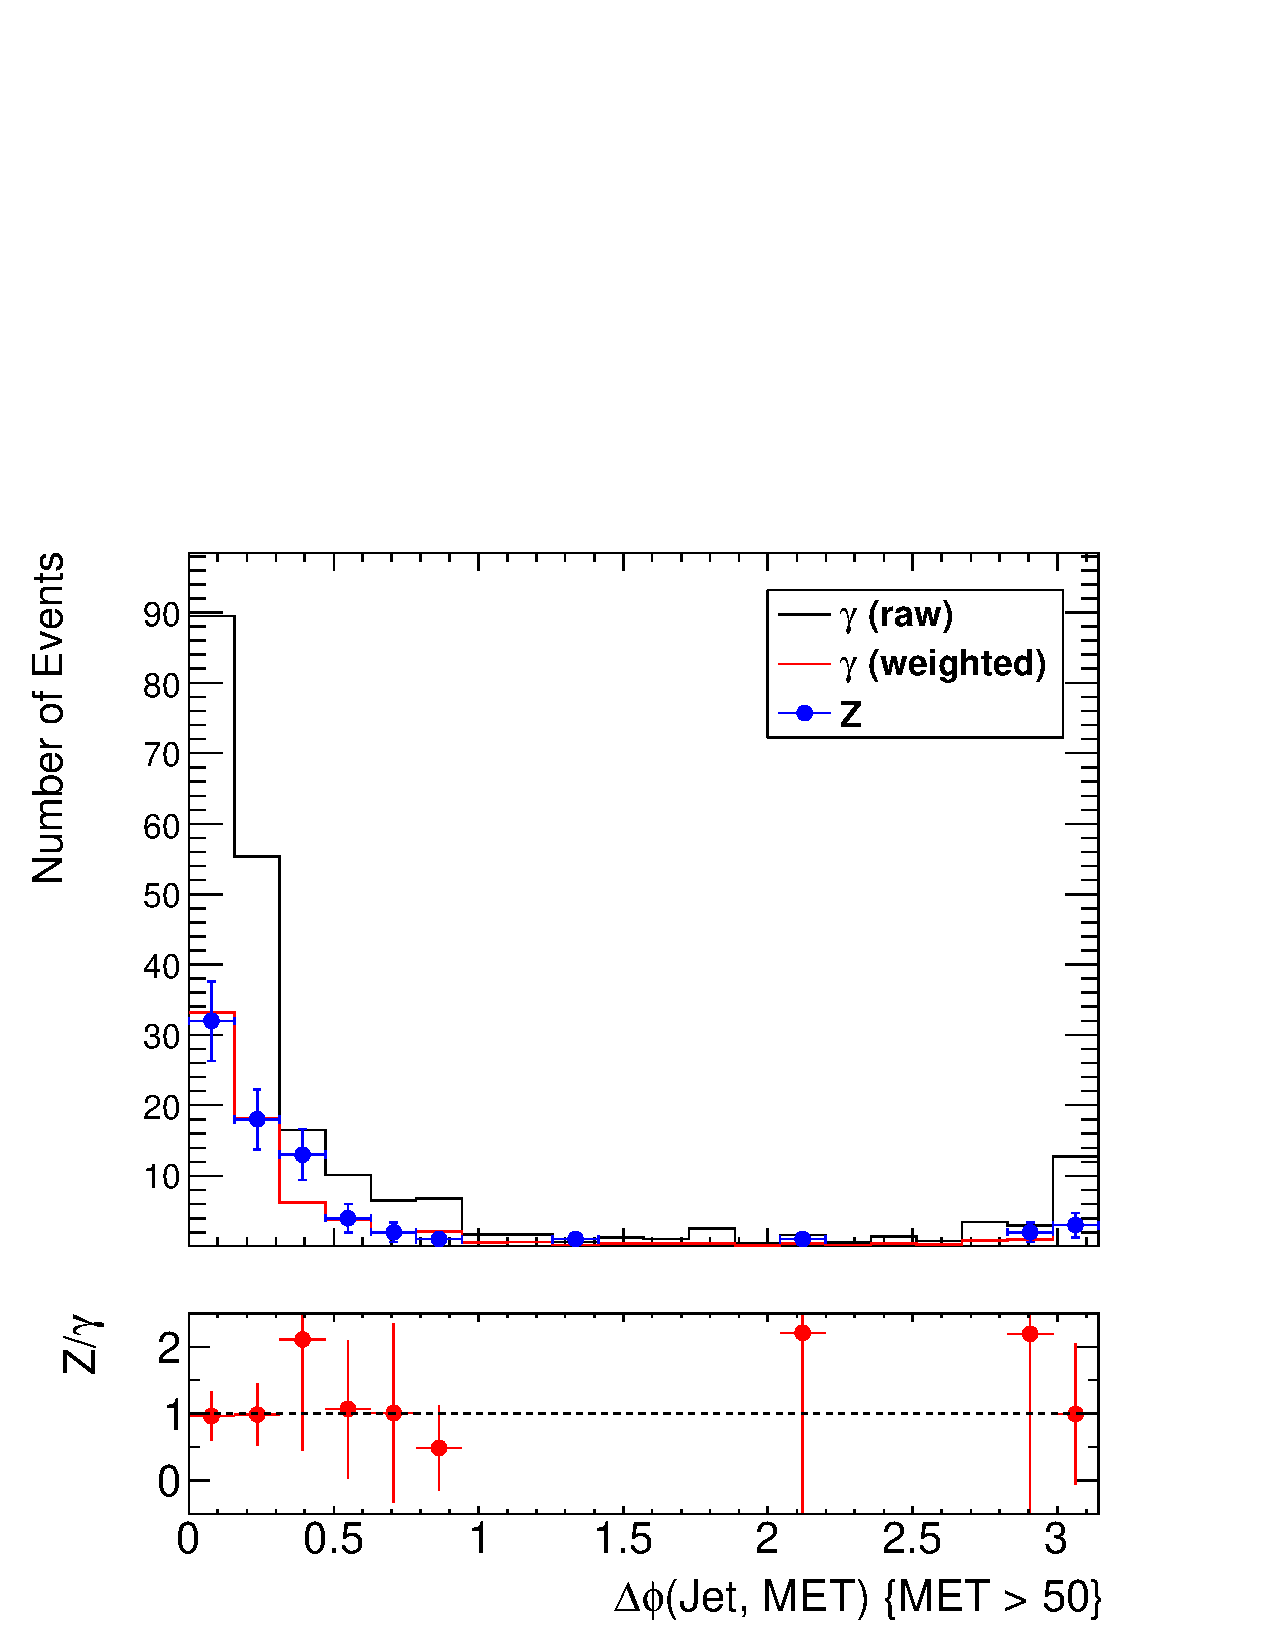
\includegraphics[width=0.49\textwidth]{figures/results_met_41X_MC_all_incl_dphi.pdf}}
\caption{Comparison of the minimum $\Delta\phi$ between the \met and the closest jet with $p_{T}>30$ GeV
in the event between the reweighted $\gamma$+jets sample and the 
simulation prediction from the $Z$+jets sample.}
\label{fig:PhotonJetsClosureTest_DPhi}
\end{center}
\end{figure}


Finally, we show the comparison between the predicted transverse mass distribution and the simulation
distribution with no cut on minimum \met in Fig \ref{fig:PhotonJetsClosureTest_MtHZZ_NoMetCut} and 
with a minimum \met cut of greater than $40$GeV in Fig \ref{fig:PhotonJetsClosureTest_MtHZZ_MetPresel}. 
The predicted shape and the simulation shape are again in reasonable agreement. 

%\begin{figure}[!htbp]
%\begin{center}
%\subfigure[0-Jet]{\includegraphics[width=0.4\textwidth]{figures/results_met_41X_MC_all_0j_mt.pdf}}
%\subfigure[1-Jet]{\includegraphics[width=0.4\textwidth]{figures/results_met_41X_MC_all_1j_mt.pdf}}
%\subfigure[2-Jet]{\includegraphics[width=0.4\textwidth]{figures/results_met_41X_MC_all_2j_mt.pdf}}
%\subfigure[Inclusive]{\includegraphics[width=0.4\textwidth]{figures/results_met_41X_MC_all_incl_mt.pdf}}
%\caption{Comparison of the transverse mass prediction from the reweighted $\gamma$+jets sample 
%and the simulation prediction from the $Z$+jets sample, where no \met cut has been applied.}
%\label{fig:PhotonJetsClosureTest_MtHZZ_NoMetCut}
%\end{center}
%\end{figure}

\begin{figure}[!htbp]
\begin{center}
\subfigure[0-Jet]{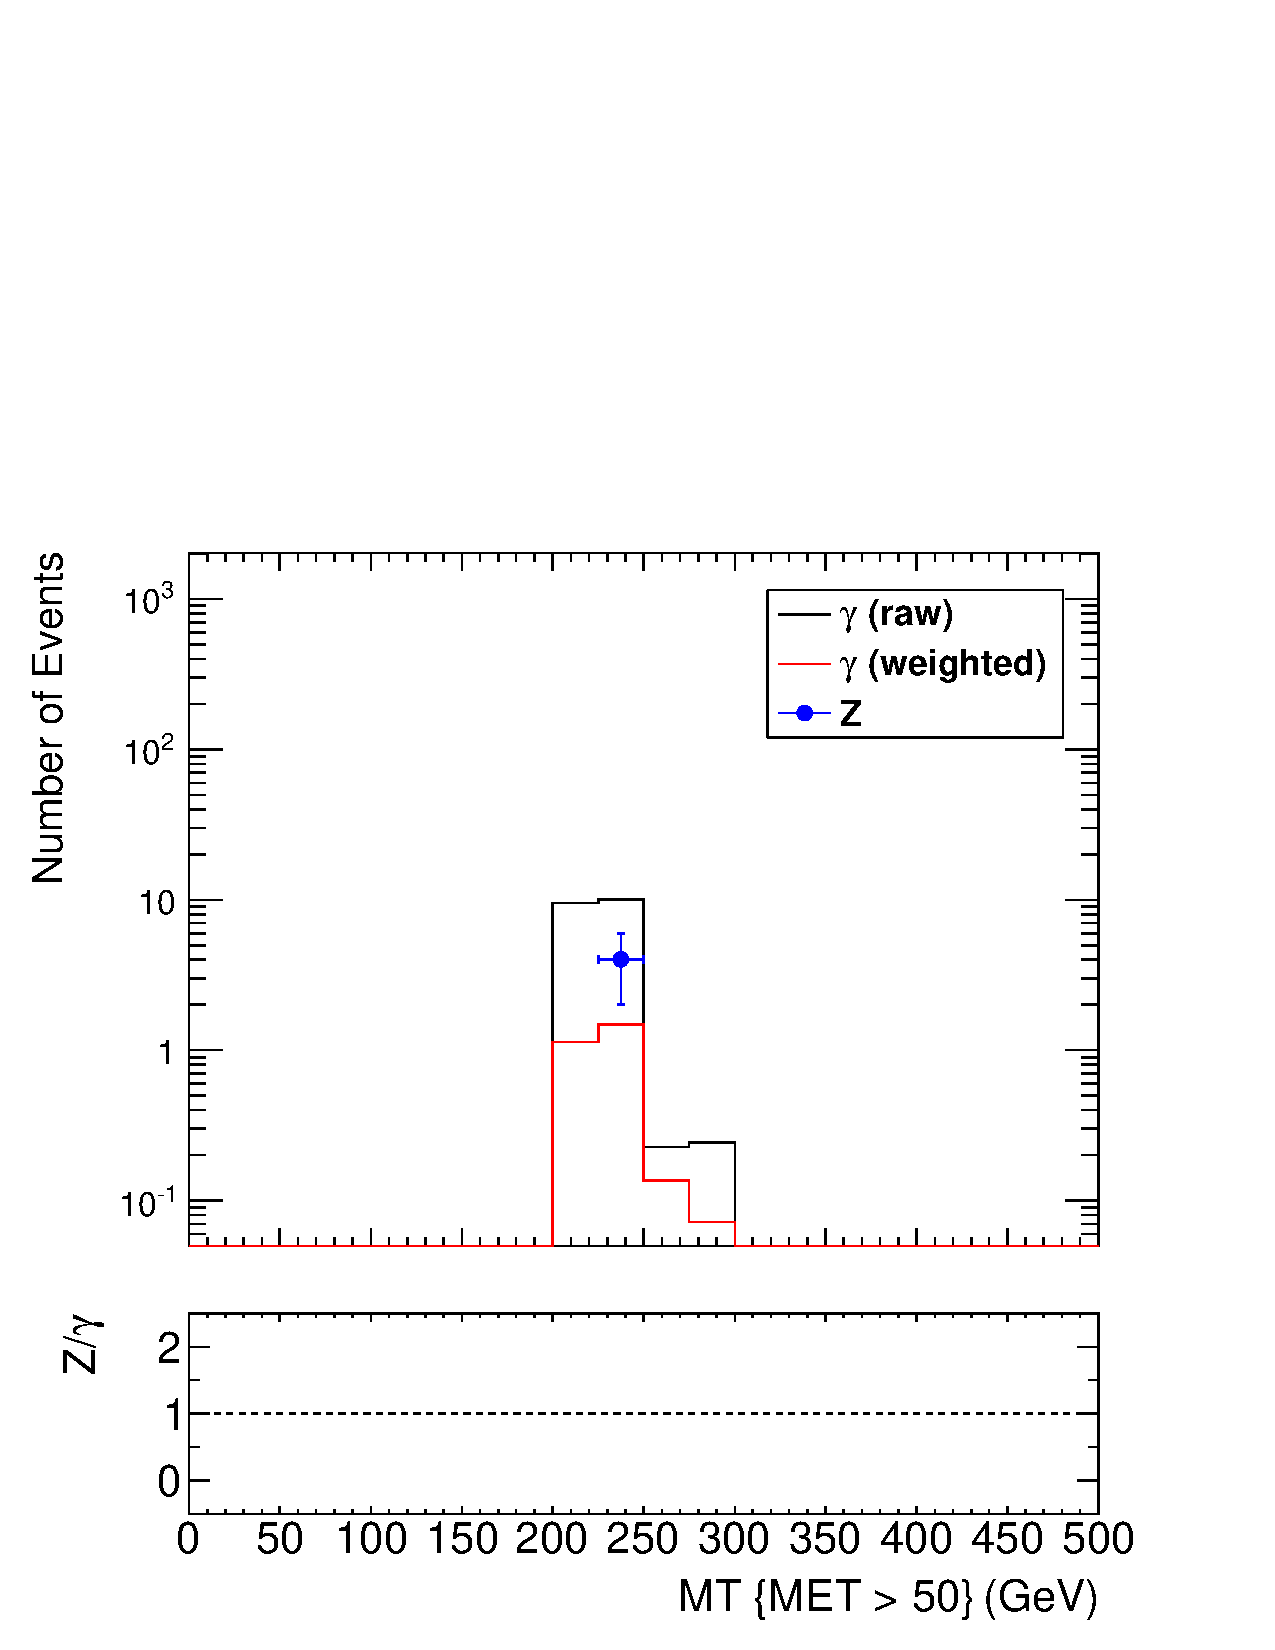
\includegraphics[width=0.49\textwidth]{figures/results_met_41X_MC_all_0j_mt_met50.pdf}}
\subfigure[1-Jet]{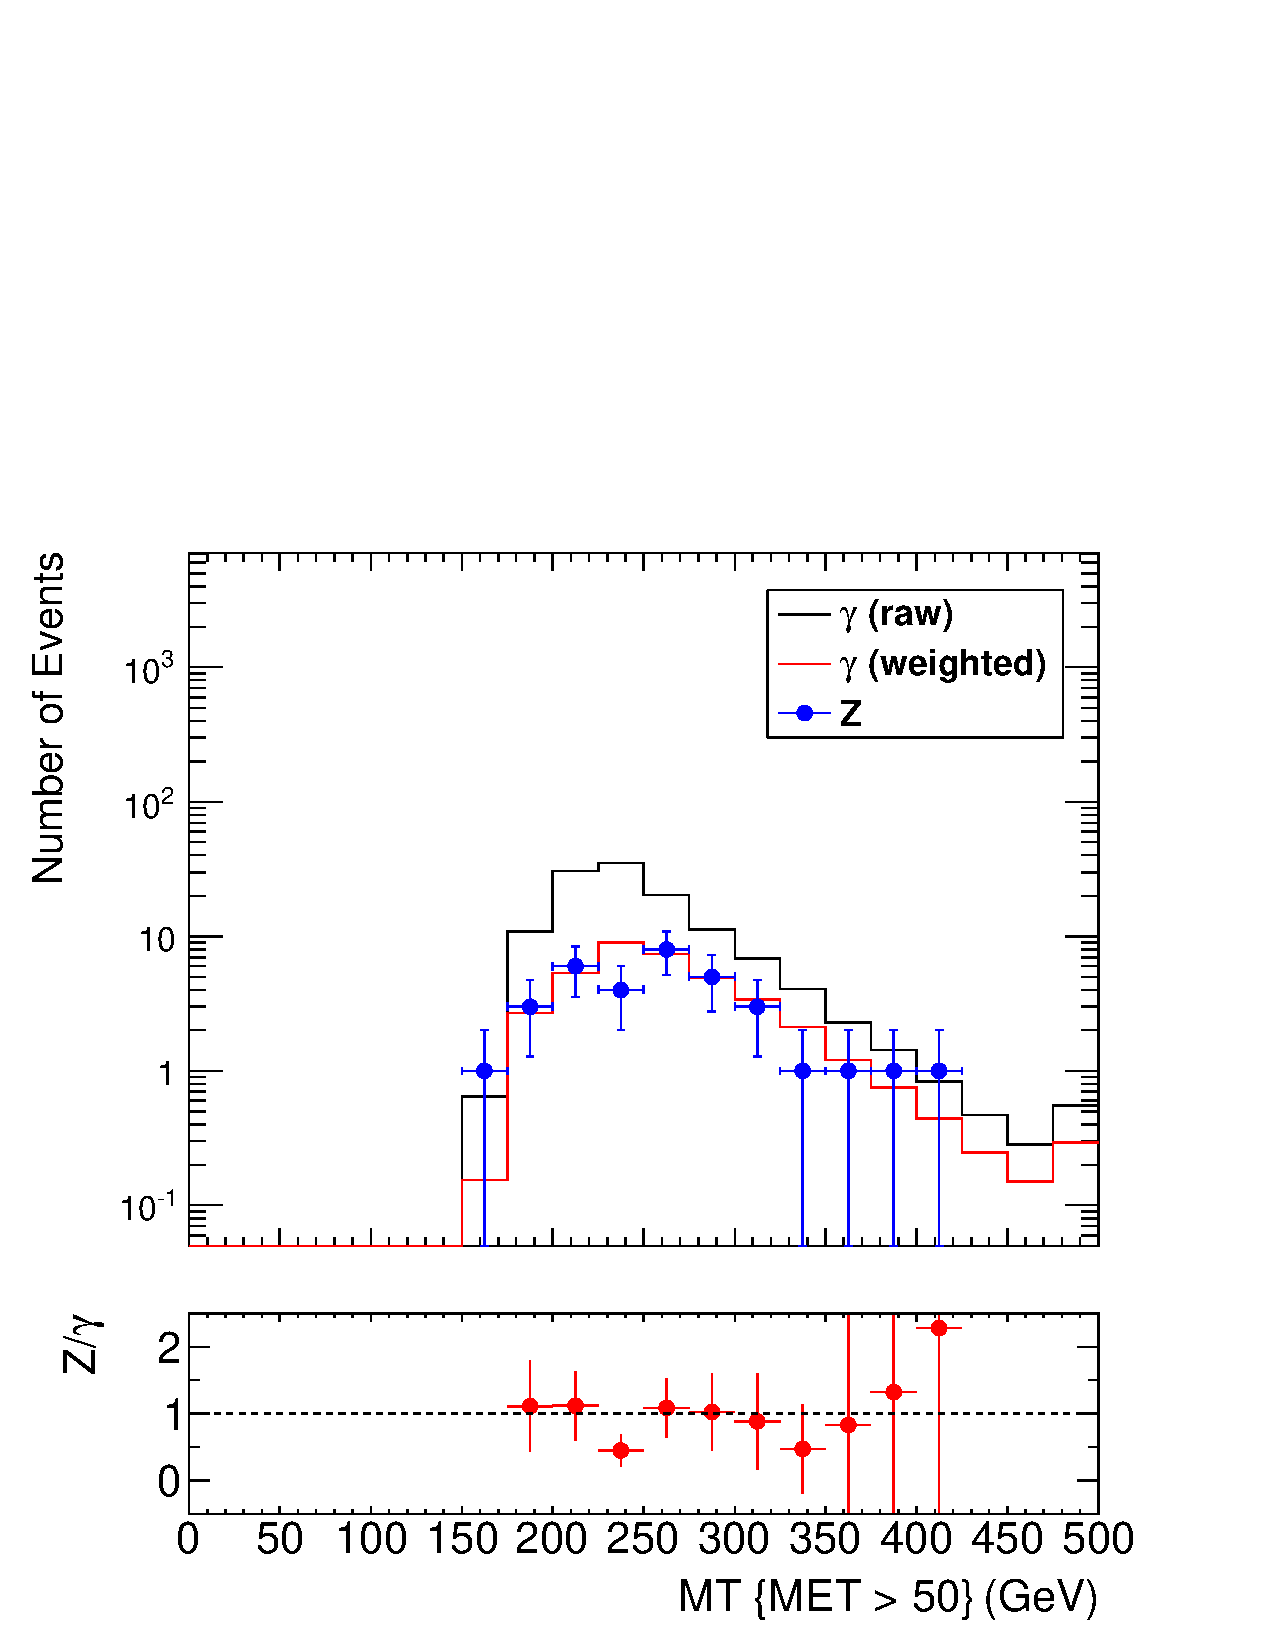
\includegraphics[width=0.49\textwidth]{figures/results_met_41X_MC_all_1j_mt_met50.pdf}}
\subfigure[2-Jet]{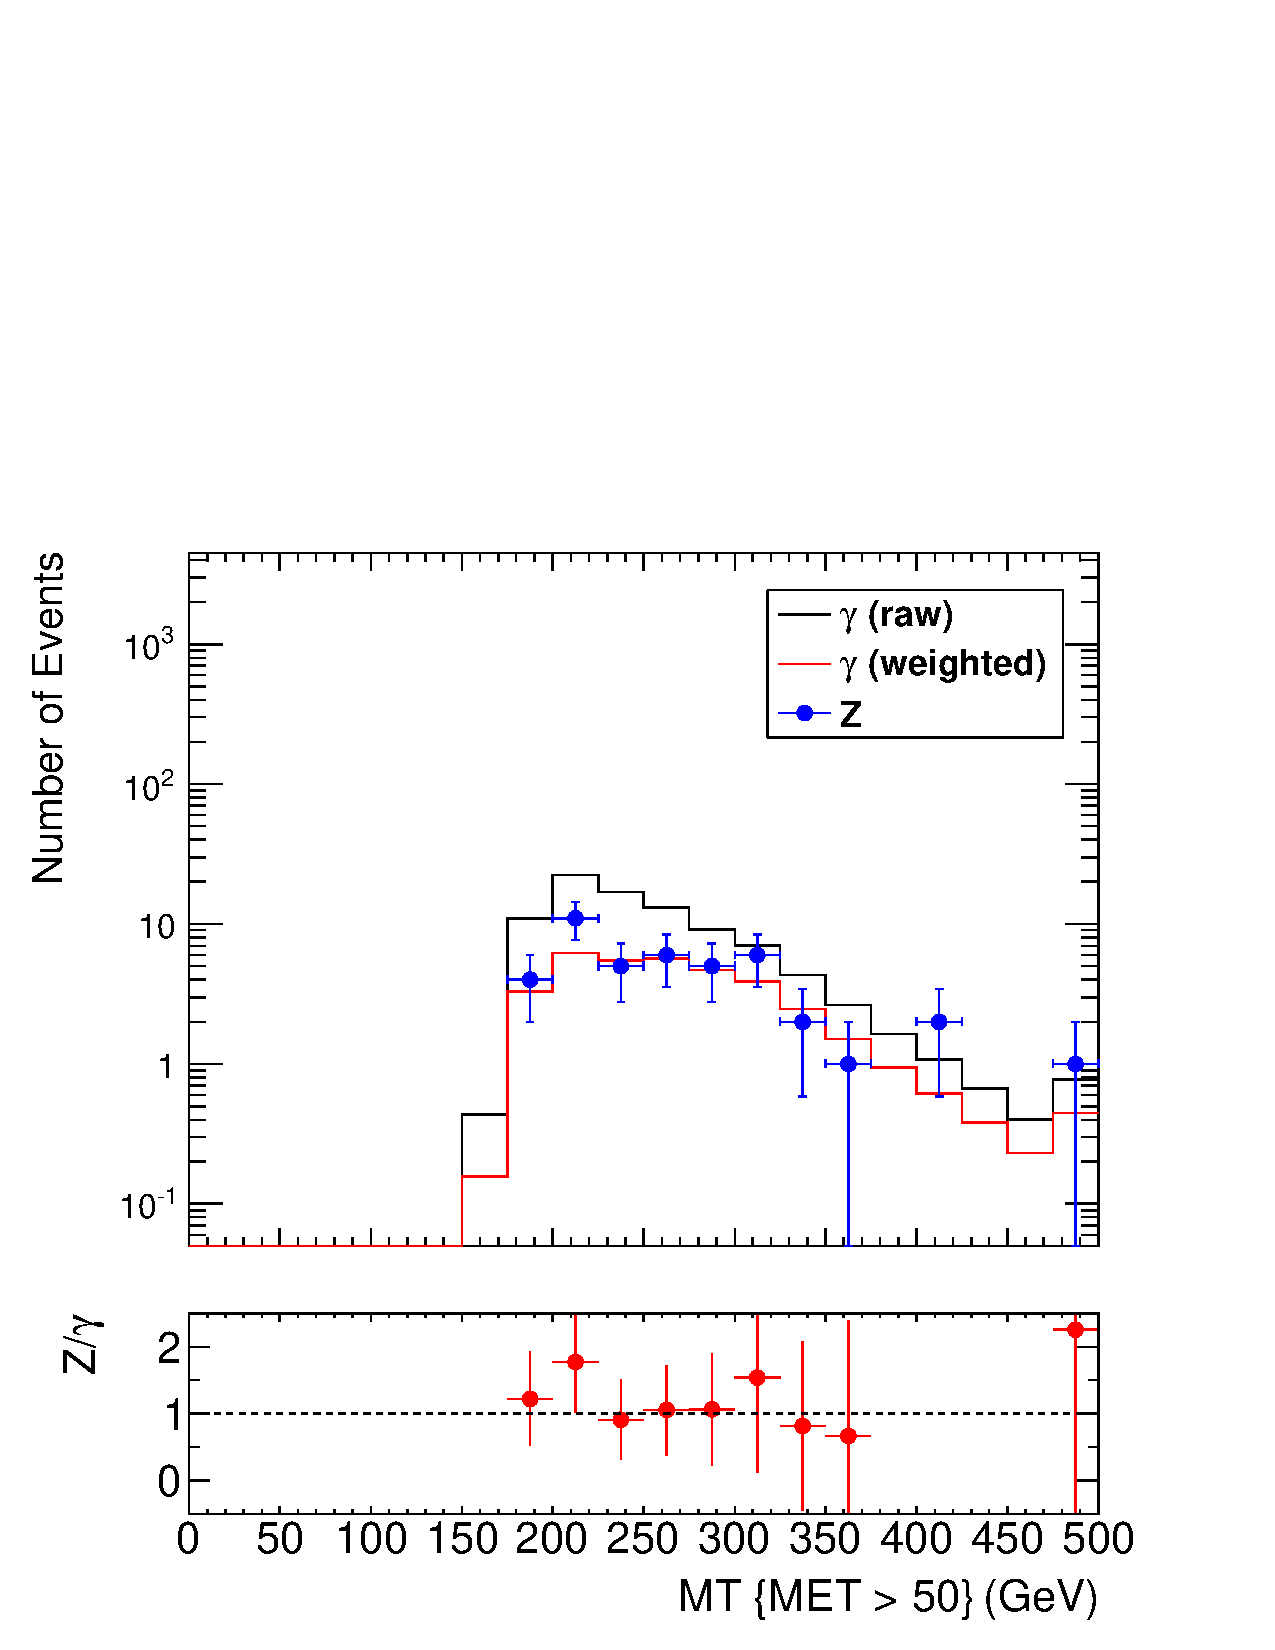
\includegraphics[width=0.49\textwidth]{figures/results_met_41X_MC_all_2j_mt_met50.pdf}}
\subfigure[Inclusive]{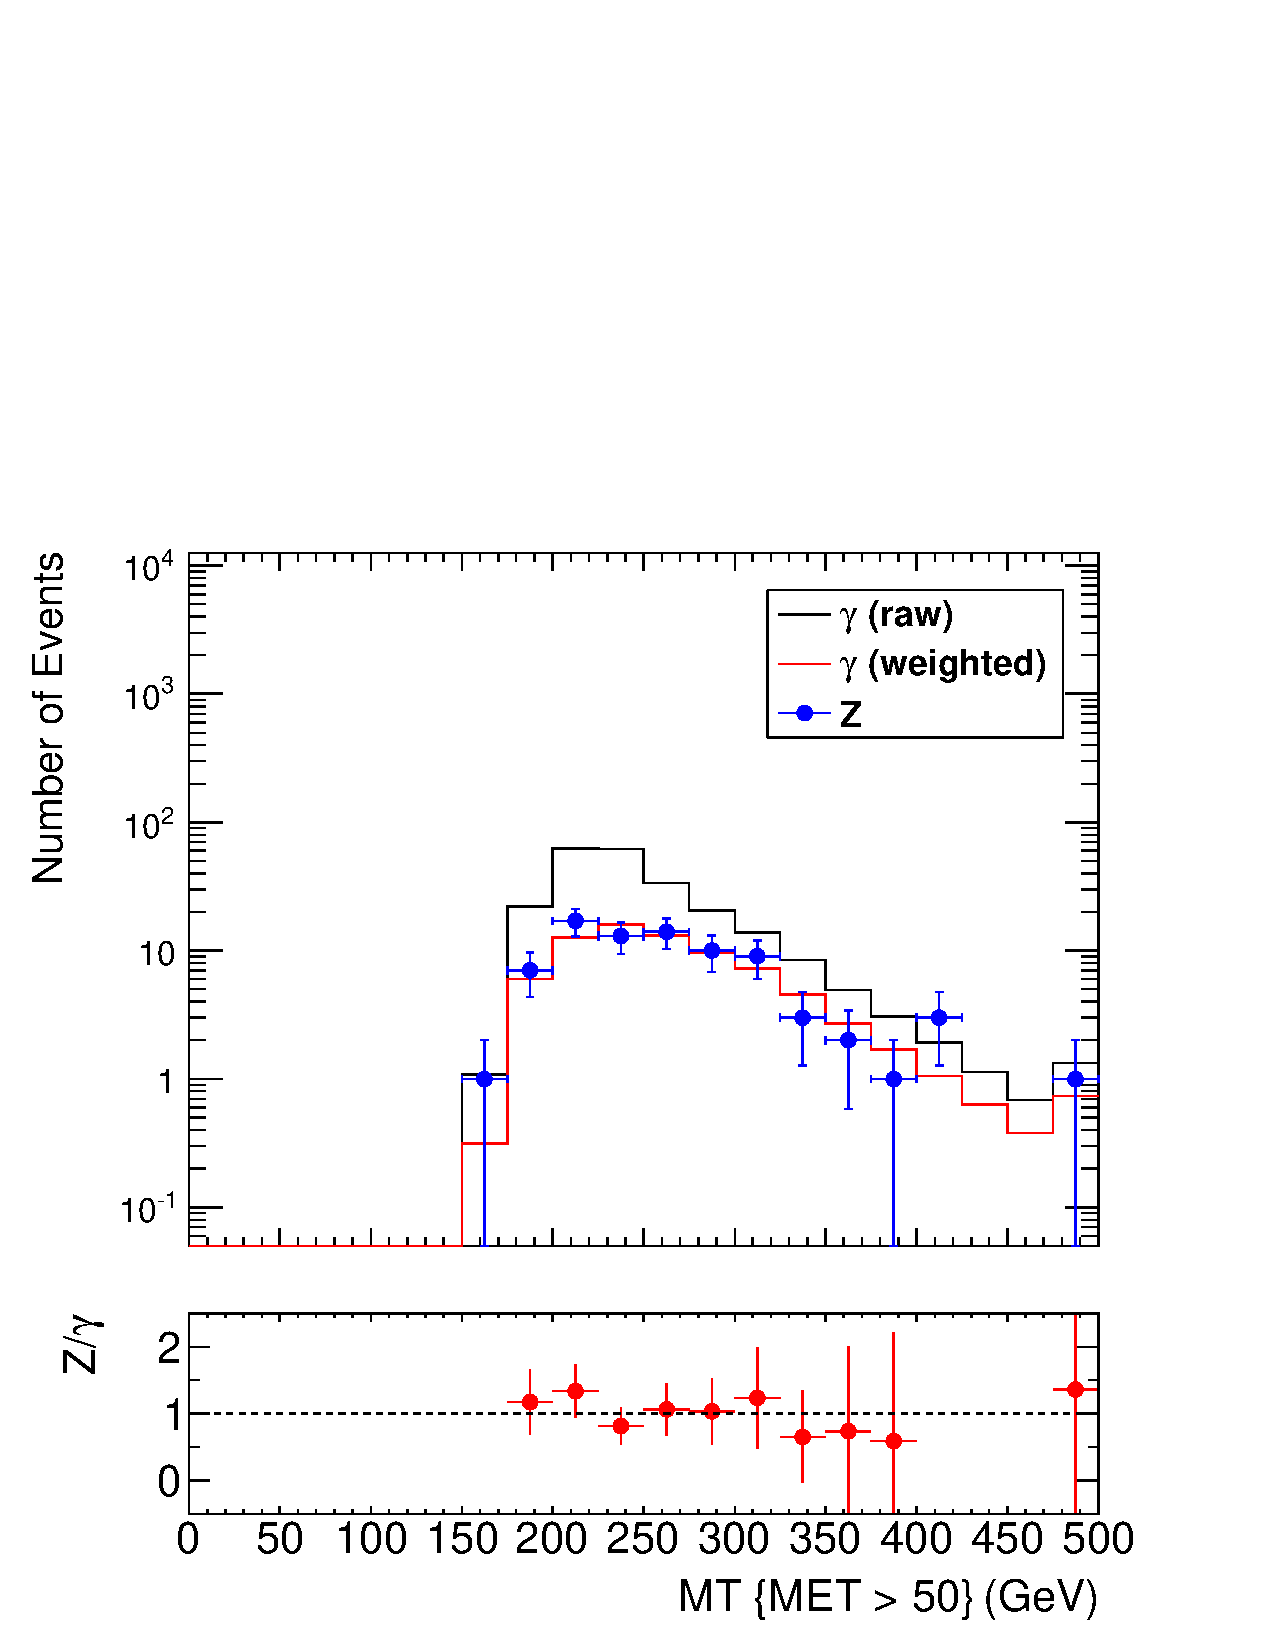
\includegraphics[width=0.49\textwidth]{figures/results_met_41X_MC_all_incl_mt_met50.pdf}}
\caption{Comparison of the transverse mass prediction from the reweighted $\gamma$+jets sample 
and the simulation prediction from the $Z$+jets sample, where the minimum \met is required to be larger than 
$40$ GeV.}
\label{fig:PhotonJetsClosureTest_MtHZZ_MetPresel}
\end{center}
\end{figure}

%
%
\subsubsection{Systematic Uncertainties}

We account for the intrinsic systematic uncertainty on the method by comparing
the predicted and observed \met~distribution in the closure test described above.
This is illustrated in Figure \ref{fig:PhotonJetsClosureTest_MinMETRatio}.
From this we conclude a systematic uncertainty of 14\% in the inslusive bin, relevant for this analysis.

\begin{itemize}
    \item TODO:
    \begin{itemize}
        \item this systematic uncertainty is itself fairly uncertain.
As mentioned before, to be repeated in 42X MC.  For now old value of 25\% still used in cards.
    \end{itemize}
\end{itemize}

%\begin{figure}[!htbp]
%\begin{center}
%\subfigure[0-Jet]{\includegraphics[width=0.4\textwidth]{figures/results_met_41X_MC_all_0j_metratio.pdf}}
%\subfigure[1-Jet]{\includegraphics[width=0.4\textwidth]{figures/results_met_41X_MC_all_1j_metratio.pdf}}
%\subfigure[2-Jet]{\includegraphics[width=0.4\textwidth]{figures/results_met_41X_MC_all_2j_metratio.pdf}}
%\subfigure[Inclusive]{\includegraphics[width=0.4\textwidth]{figures/results_met_41X_MC_all_incl_metratio.pdf}}
%\caption{
%The ratio of the \met prediction from
%the reweighted $\gamma$+jets sample and the simulation prediction from the $Z$+jets sample.}
%\label{fig:PhotonJetsClosureTest_MinMETRatio}
%\end{center}
%\end{figure}


%\subsubsection{Data Estimate}
%
%We compared the predictions for the minimum \met and MT are compared with the  
%data at the \zz preselection level to validate the method.
%These comparisons are shown in Section \ref{sec:dataresults} in
%Figures \ref{fig:minmet_zzpresel} and \ref{fig:mt_zzpresel} respectively.
%This is done sparately for the 0-jet, 1-jet and 2-jet bins. 
%Including all of the backgrounds with real \met, we find reasonable agreement with data. 
%Based on the $\gamma$+jet sample prediction, we obtain the background predictions for the
%preselection and all the mass dependent cut-based analyses summarized in Table \ref{tab:DYBkgPrediction}.
%
%\begin{table}[!htbp]
%\begin{center}
%{\footnotesize
%\begin{tabular}{|l|c|c|c|c|}
%\hline
%Higgs Mass      &  0-jet bin             & 1-jet bin             & 2-jet bin             & Total                \\
%\hline
%ZZ Preselection &  $16.34\pm1.59\pm4.1$  & $17.57\pm1.59\pm3.51$      & $99.10\pm1.60\pm20.81$ & $133.0\pm2.76\pm21.50$ \\ \hline
%250             &  $6.73\pm0.39\pm1.68$  & $4.76\pm0.38\pm0.95$       & N/A                    & $11.49\pm0.54\pm1.93$\\
%300             &  $0.51\pm0.16\pm0.13$  & $0.33\pm0.15\pm0.06$       & N/A                    & $0.84\pm0.22\pm0.14$\\
%400             &  $0.00\pm0.07\pm0.00$  & $0.87\pm0.10\pm0.17$       & N/A                    & $0.87\pm0.12\pm0.17$\\
%\hline
%\end{tabular}
%}
%\caption{Summary of $Z$+jets background yields estimated using $\gamma$+jets events in 1092 $\ipb$. Both statsitical and 
%systematic uncertainties are reported.}
%\label{tab:DYBkgPrediction}
%\end{center}
%\end{table}

